% Supplementary figure captions: MCMC chain and run agreement
% ClonalGE applied to the prostate cancer dataset (10 independent runs,
% 10 parallel MCMC chains per run).
%
% ── Generation pipeline (shared across all figures) ───────────────────────────
%
% Step 1 — Within-run chain selection.
%   For each run, the chain with the highest log-likelihood is identified as
%   the within-run reference.  All other chains in that run are aligned to the
%   reference by computing the Pearson correlation of their flattened inferred_H
%   vectors.  Chains with r > 0.9 are retained; the rest are discarded.
%   The within-run posterior estimate for that run is the element-wise mean of
%   the retained chains' inferred_H, inferred_B, and inferred_n arrays.
%
% Step 2 — Cross-run consensus selection (Hungarian clone alignment).
%   Because mixture models are invariant to relabelling of latent components,
%   clone indices may differ across runs.  For each candidate reference run,
%   every other run's per-run H matrix is realigned to the reference using the
%   Hungarian algorithm: a K×K cost matrix of negative Pearson correlations
%   between clone columns is constructed and minimised with the linear
%   assignment solver, yielding the optimal clone permutation.  The same
%   permutation is applied to B.
%   After alignment, the number of runs that agree with the candidate reference
%   (r > 0.9 on the flattened aligned H) is counted.  The candidate that
%   maximises this count — the consensus run — is chosen as the final
%   reference.  Ties are broken by the highest mean r among agreeing runs.
%   The final posterior estimates of H and B are the element-wise means of the
%   aligned H and B arrays from all runs in the consensus group.

% ── Figure S1: within-run chain agreement, best-loglik run ───────────────────
\begin{figure}[htbp]
  \centering
  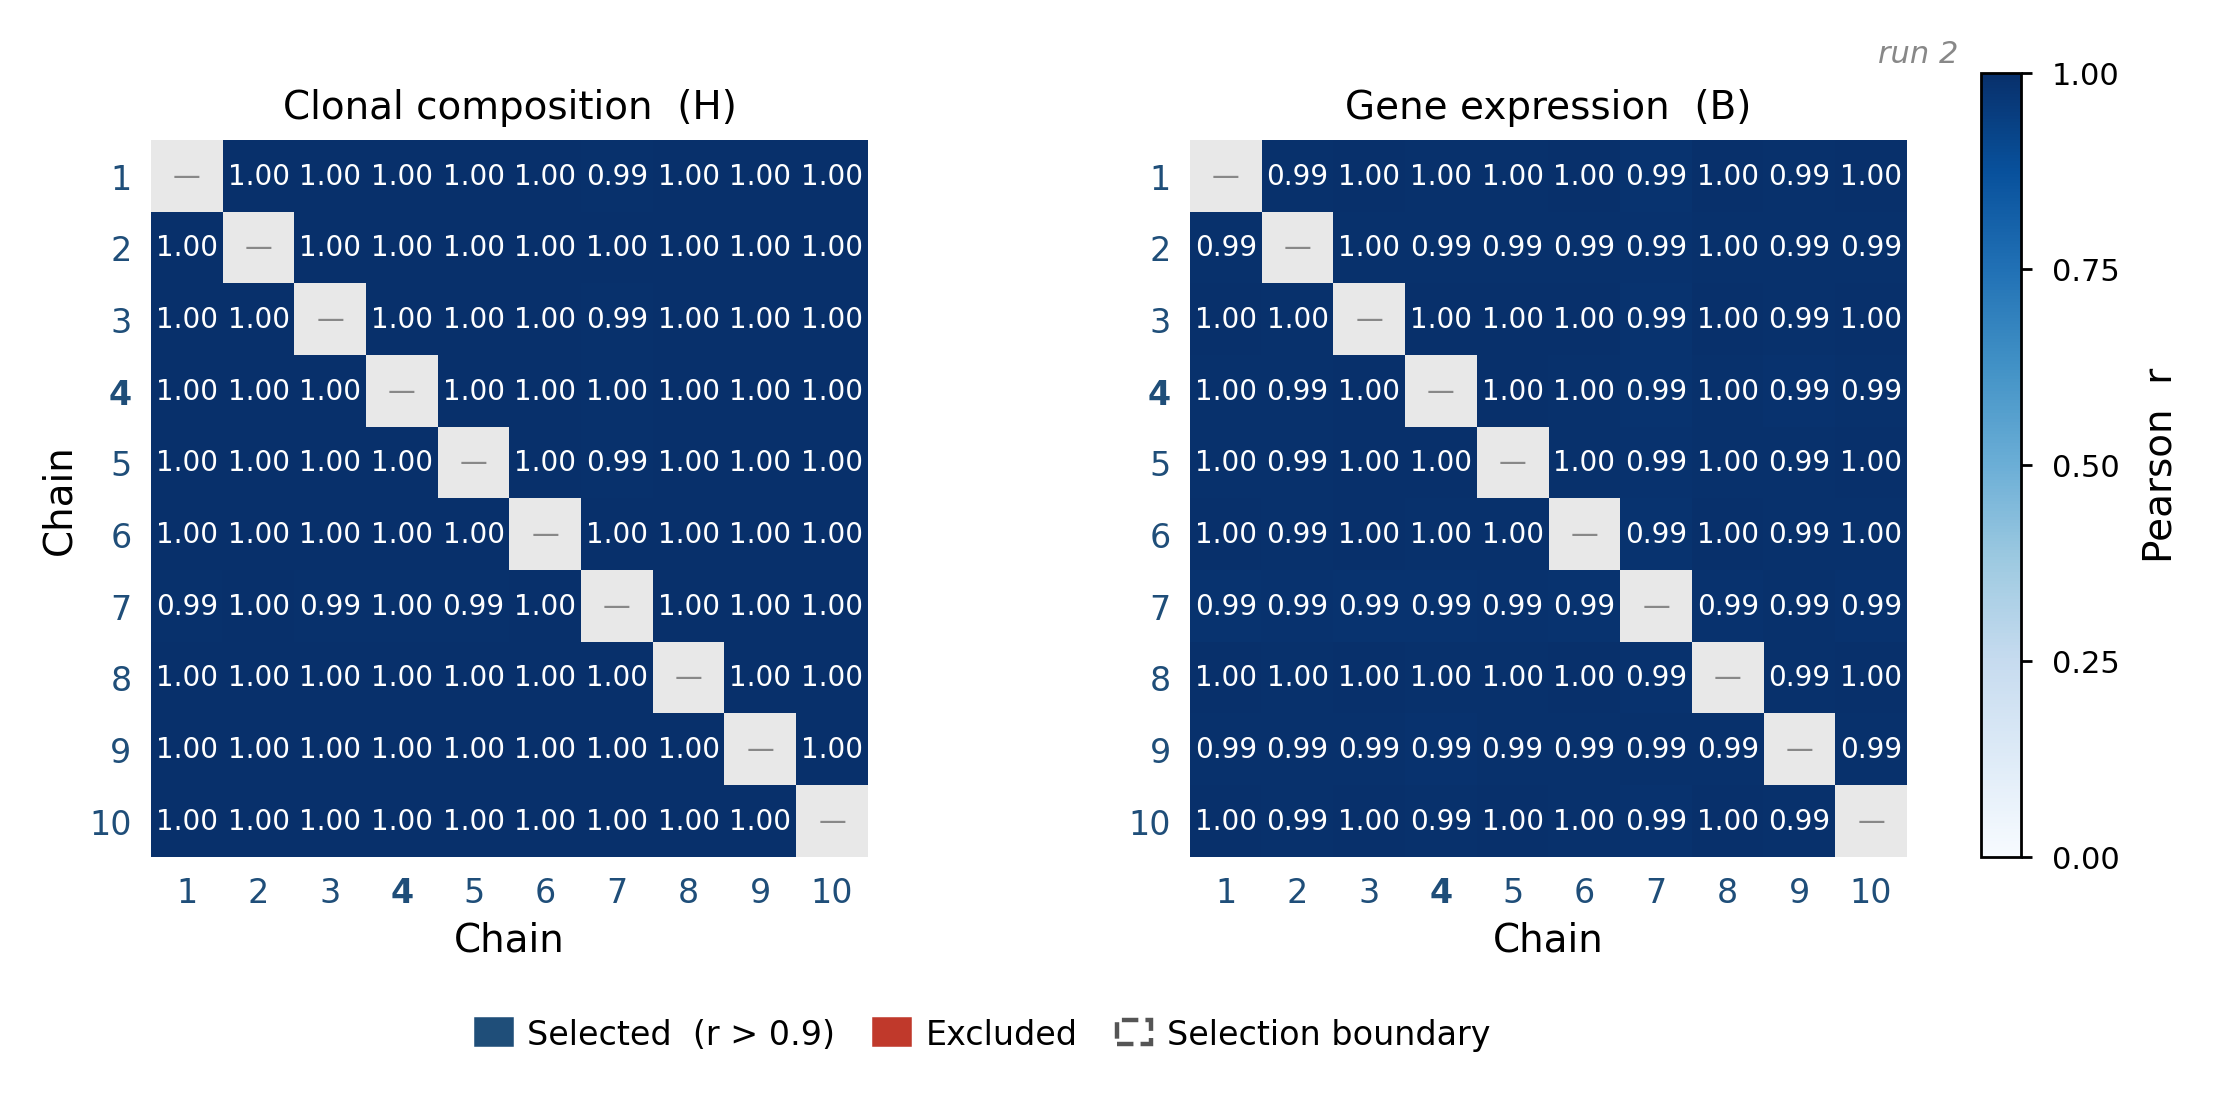
\includegraphics[width=0.75\textwidth]{plots_paper/chain_agreement.png}
  \caption{%
    \textbf{Within-run MCMC chain agreement for the run with the highest
    log-likelihood (run~2).}
    %
    \textit{Generation.}
    All ten chains from run~2 were loaded.
    For each pair of chains $(i, j)$, the Pearson correlation between the
    flattened posterior mean arrays \texttt{inferred\_H} and
    \texttt{inferred\_B} was computed, giving two symmetric $10 \times 10$
    correlation matrices.
    Chains were reordered so that those retained by the within-run selection
    criterion ($r > 0.9$ against chain~4, the highest-loglik chain, bold)
    appear first; a dashed line separates selected (blue labels) from
    excluded (red labels) chains.
    %
    \textit{Result.}
    All ten chains were retained (minimum pairwise $r = 0.99$ for both $H$
    and $B$), demonstrating that independently initialised Gibbs samplers
    converge to a consistent posterior solution within a single run.%
  }
  \label{fig:chain_agreement}
\end{figure}

% ── Figure S2: within-run chain agreement, all runs ──────────────────────────
\begin{figure}[htbp]
  \centering
  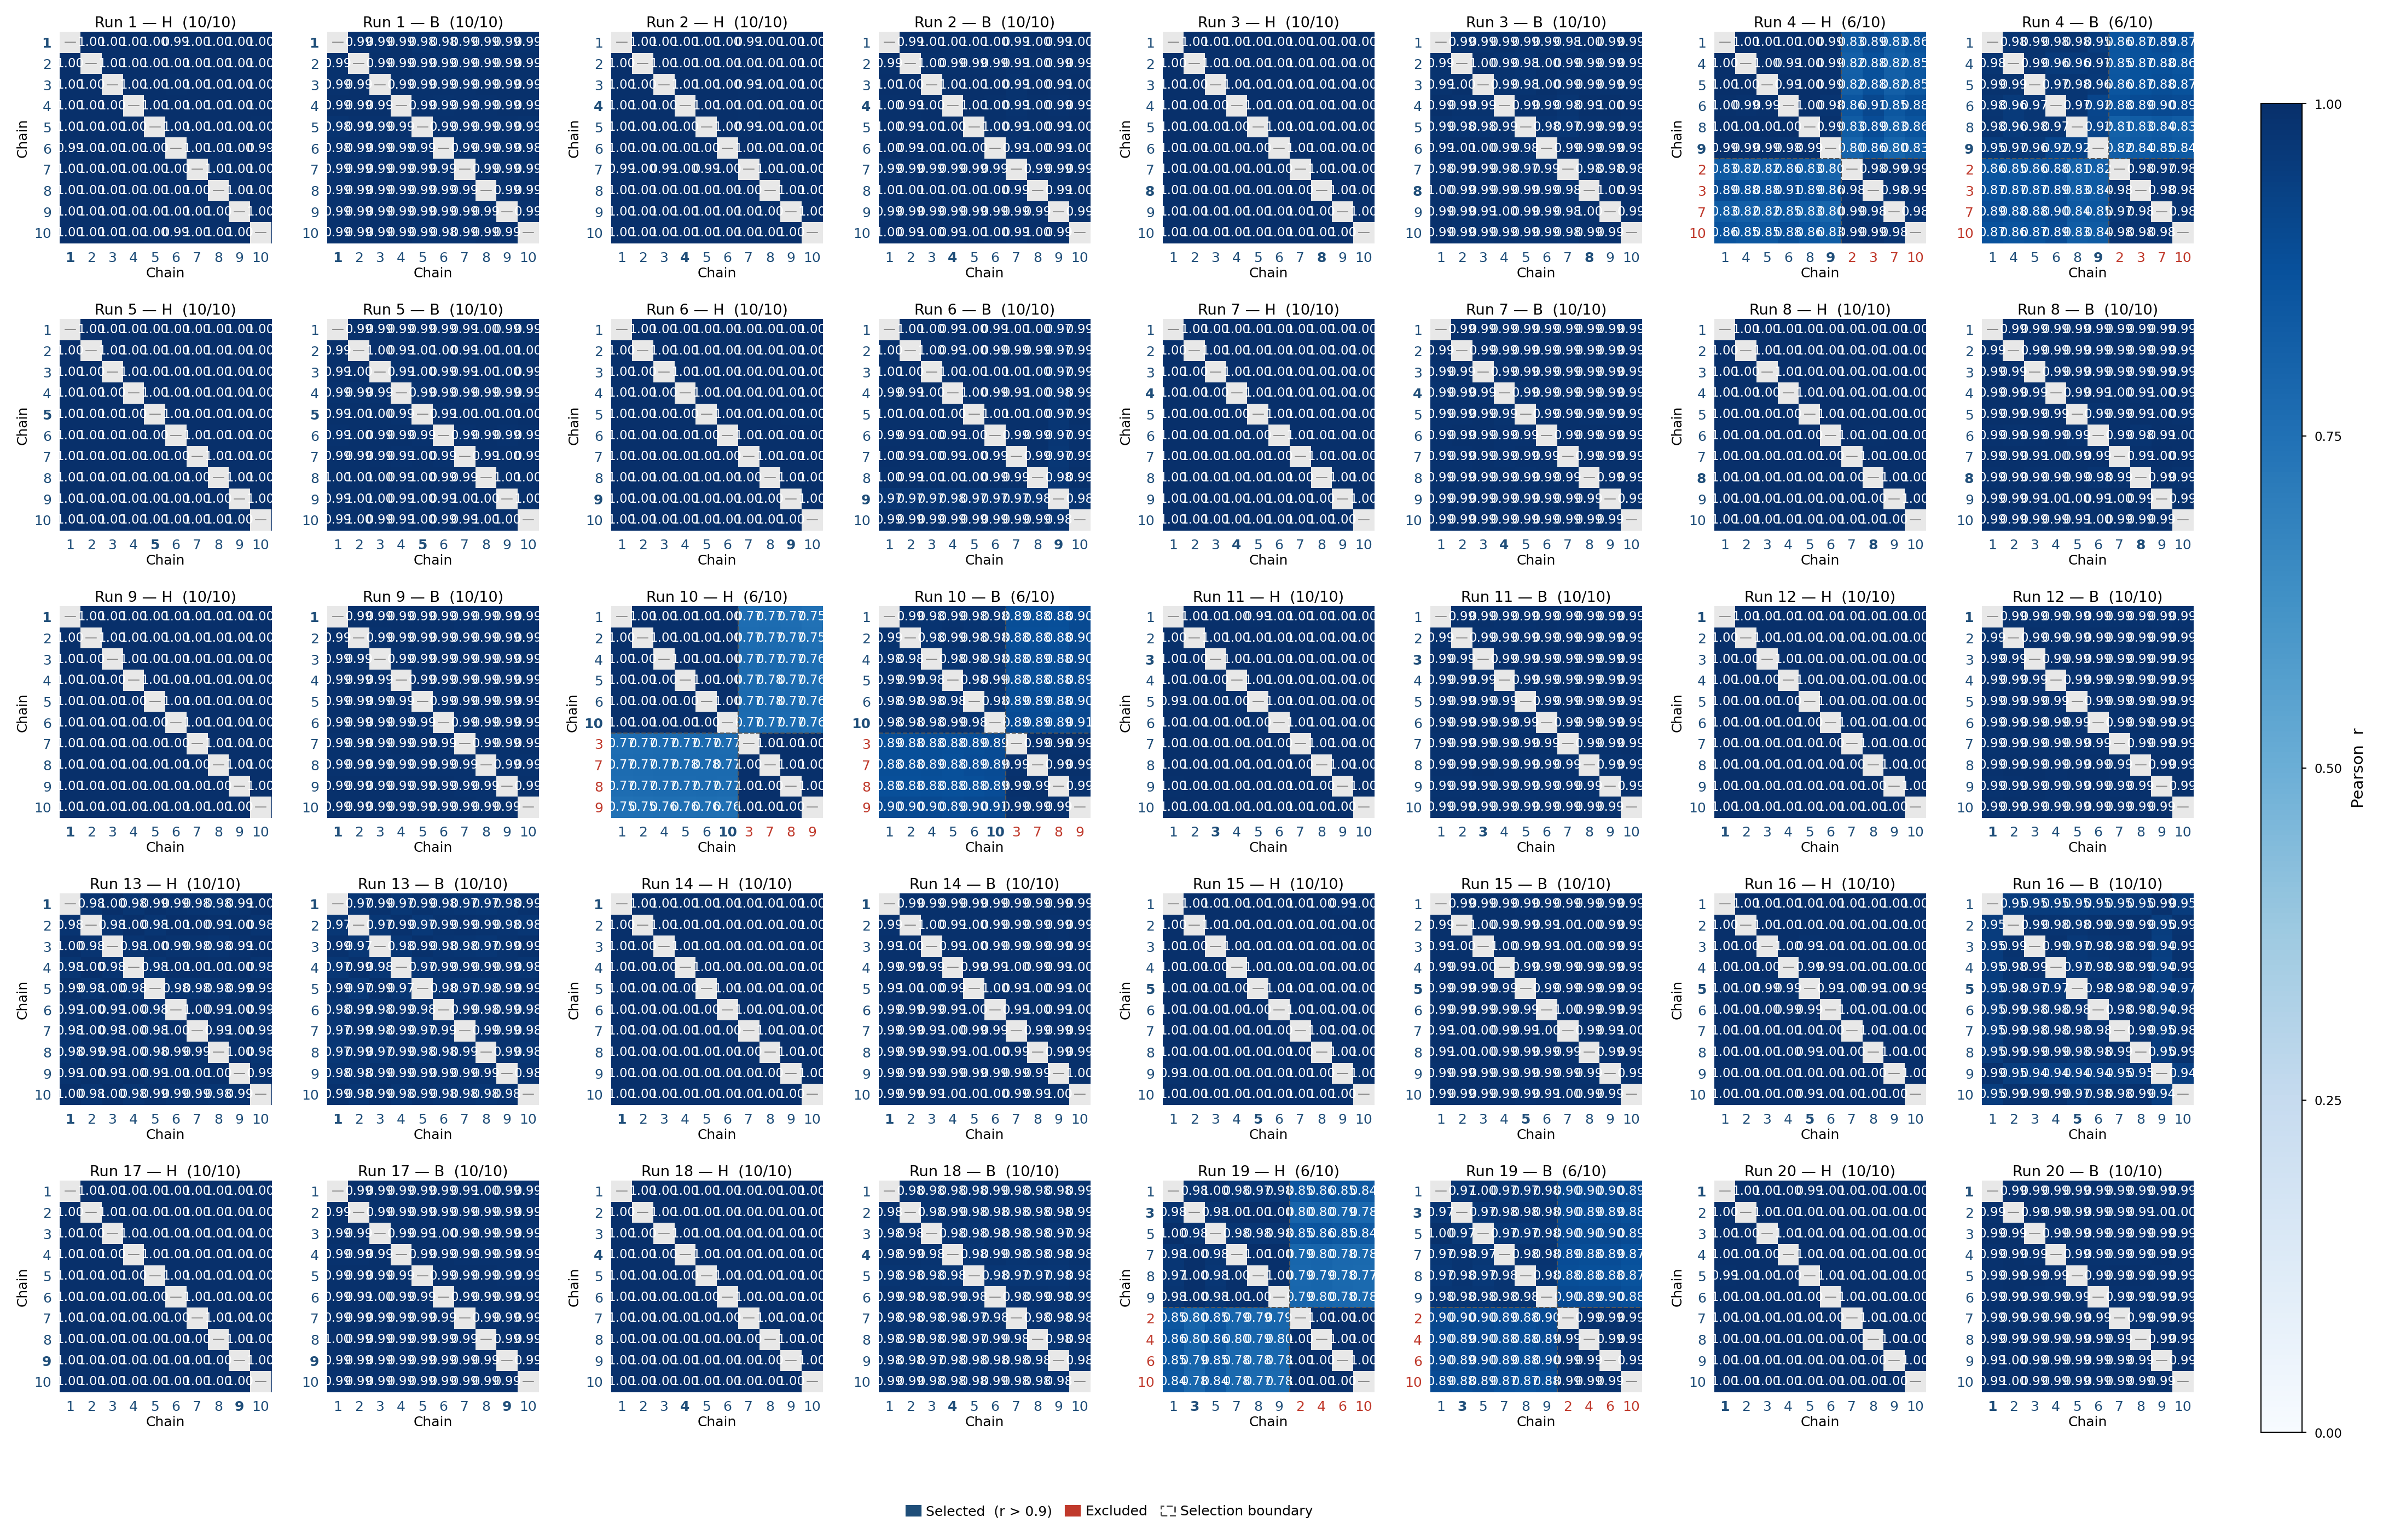
\includegraphics[width=\textwidth]{plots_paper/chain_agreement_supp.png}
  \caption{%
    \textbf{Within-run MCMC chain agreement across all ten independent runs.}
    %
    \textit{Generation.}
    The same pairwise Pearson correlation procedure described for
    Figure~\ref{fig:chain_agreement} was applied independently to each of
    the ten runs.
    Panels are arranged as a $5 \times 4$ grid: the top two heatmap rows
    show $H$ (clonal composition) and $B$ (gene expression) for runs~1--5;
    the bottom two rows show the same for runs~6--10.
    Within each panel, the highest-loglik chain (bold) serves as the
    within-run reference; chains with $r > 0.9$ against it are labelled
    in blue and placed before the dashed selection boundary, while excluded
    chains are labelled in red.
    The panel title reports the number of retained chains.
    %
    \textit{Result.}
    Nine of ten runs retained all ten chains ($10/10$); run~4 retained six
    ($6/10$), with four chains diverging to a different region of the
    posterior.
    In all runs, retained chains show pairwise $r \geq 0.97$ for $H$ and
    $r \geq 0.87$ for $B$, confirming robust within-run convergence.%
  }
  \label{fig:chain_agreement_supp}
\end{figure}

% ── Figure S3: across-run agreement ──────────────────────────────────────────
\begin{figure}[htbp]
  \centering
  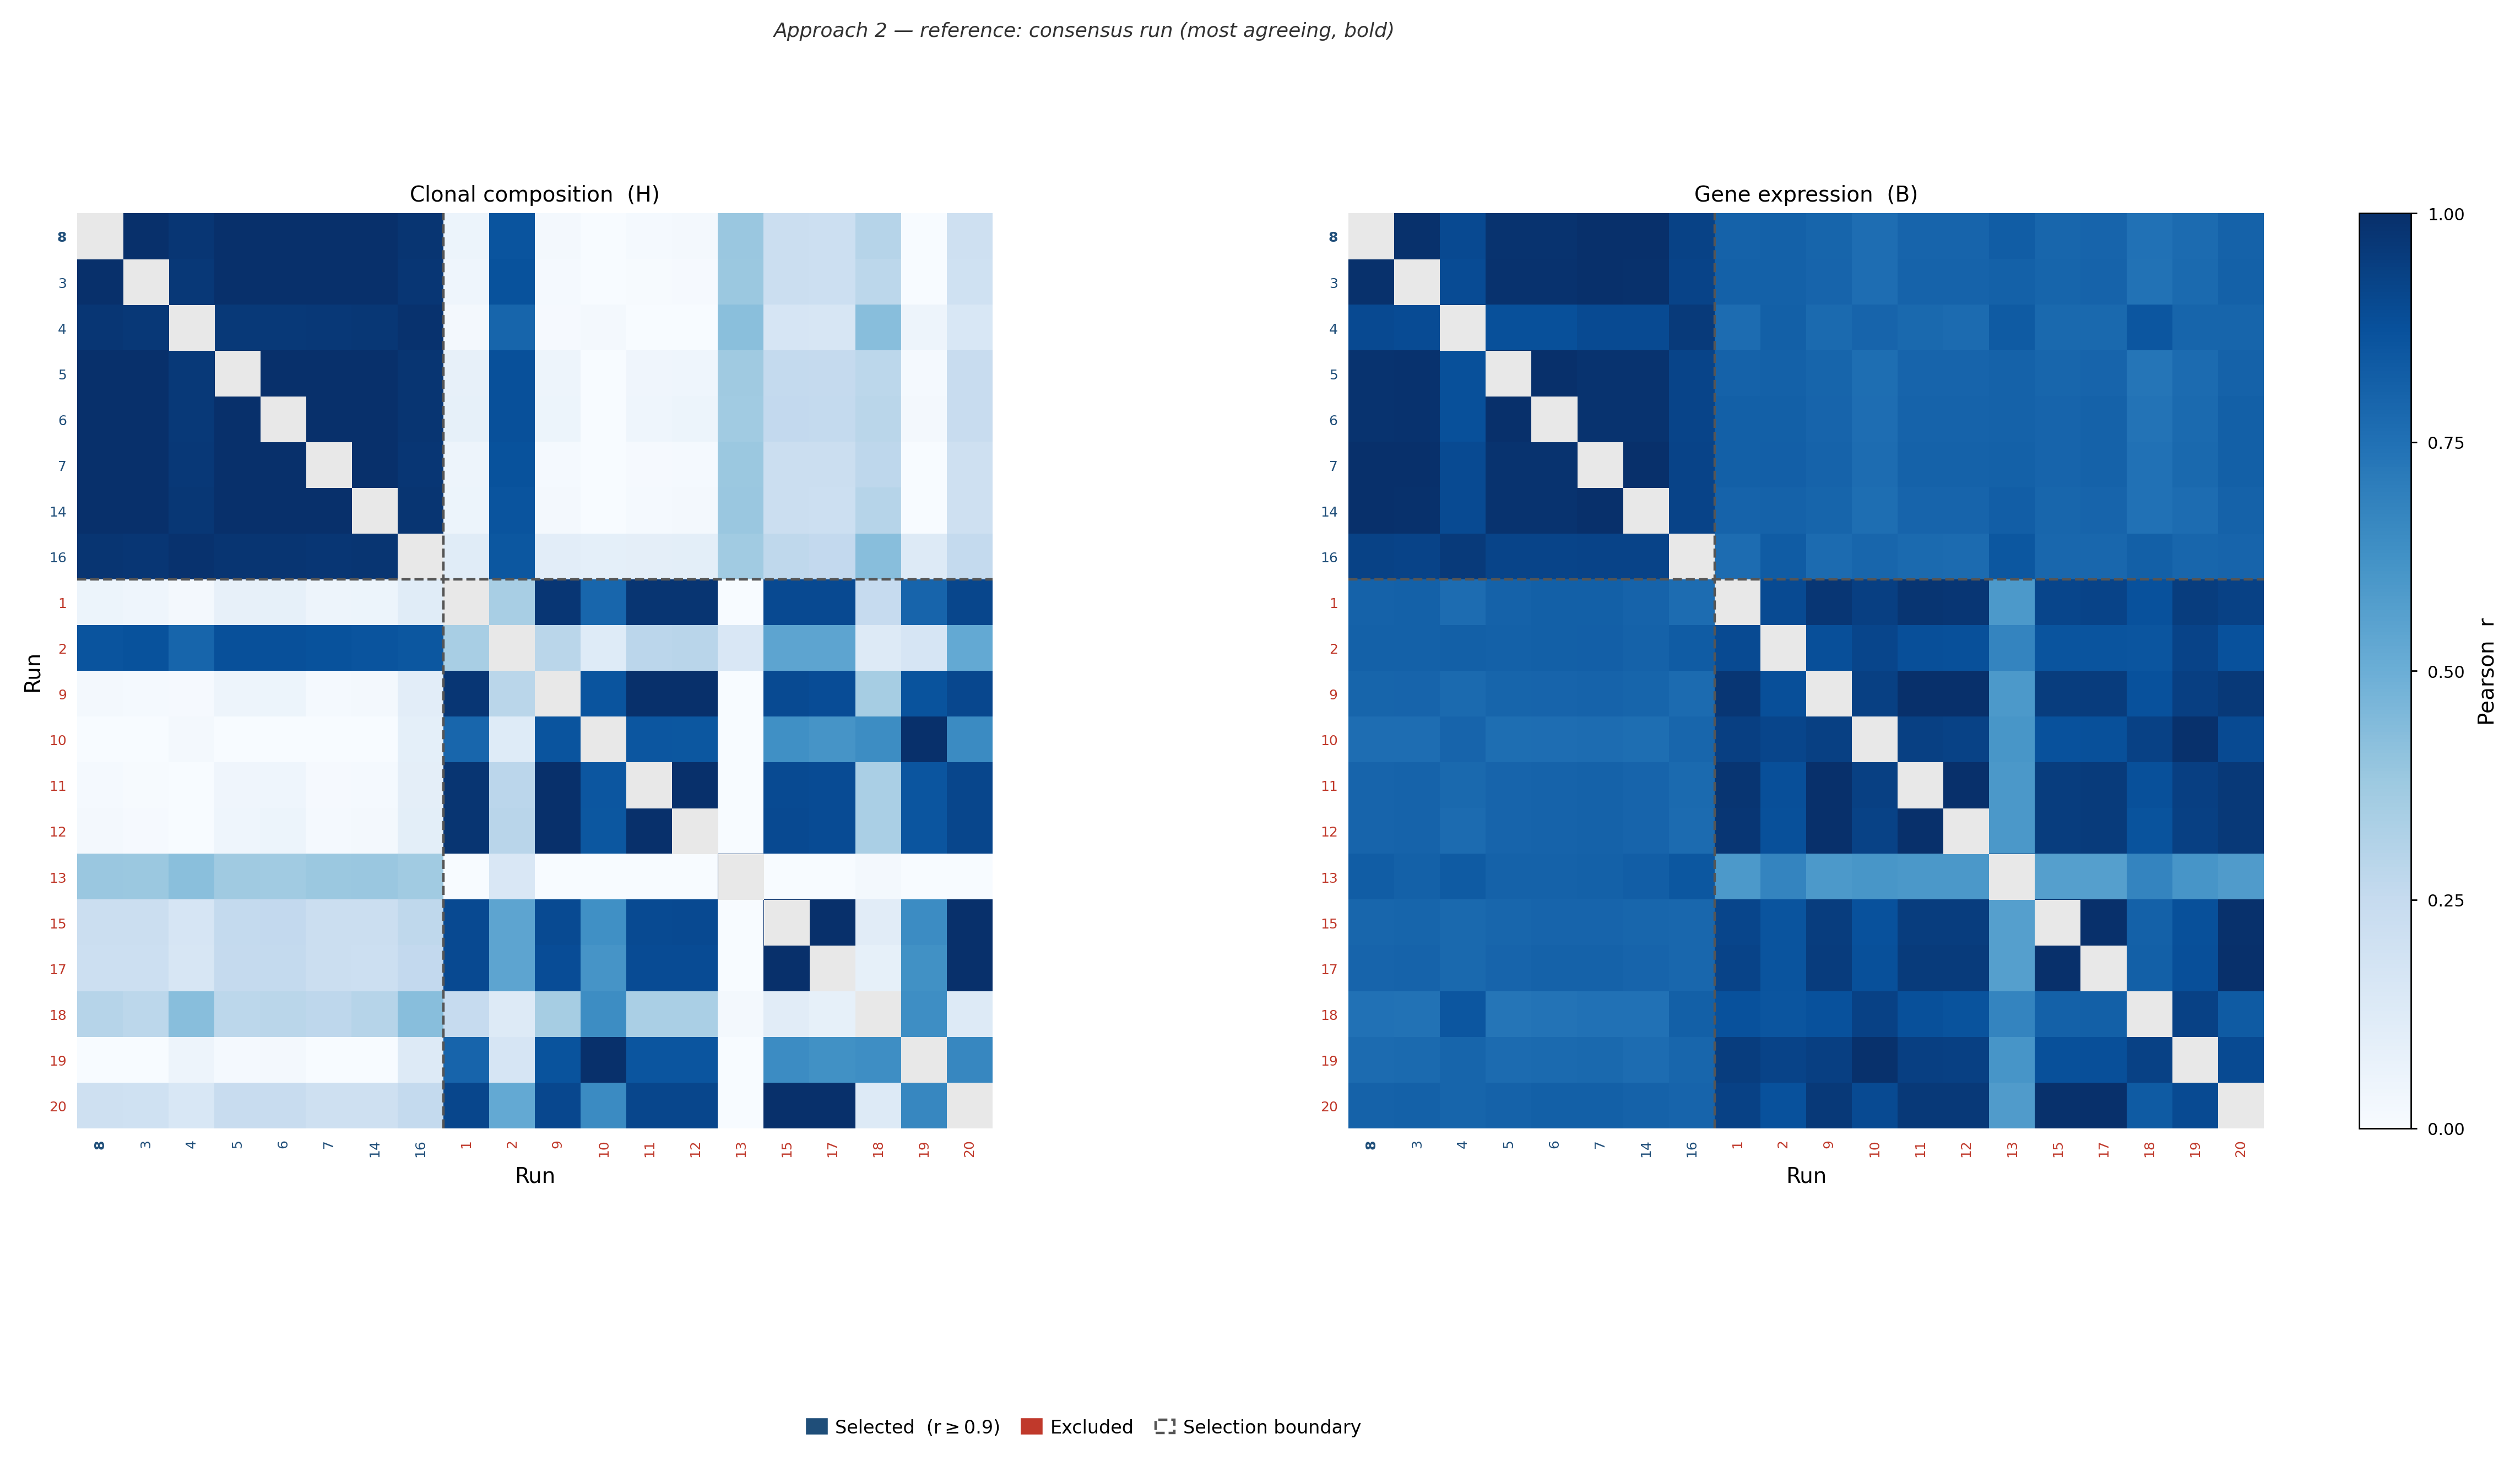
\includegraphics[width=0.75\textwidth]{plots_paper/run_agreement.png}
  \caption{%
    \textbf{Across-run agreement over ten independent runs after
    consensus-based clone alignment.}
    %
    \textit{Generation.}
    Each run's posterior estimate of $H$ and $B$ was first obtained by
    within-run chain selection and averaging (Step~1 above).
    The consensus run was then identified by the Hungarian alignment
    procedure (Step~2): run~8 maximised the number of agreeing runs after
    clone realignment, with six of ten runs satisfying $r > 0.9$ on the
    aligned $H$ (runs~3--8, blue labels).
    The $10 \times 10$ pairwise Pearson correlation matrix was computed on
    the aligned $H$ and $B$ arrays; runs are ordered with the consensus
    group first.
    %
    \textit{Result.}
    Within the selected group, mean pairwise $r = 0.99$ (minimum $0.96$)
    for $H$ and mean $r = 0.96$ (minimum $0.88$) for $B$, confirming
    reproducible recovery of clonal composition and gene expression
    structure.
    The four excluded runs (red labels, runs~1, 2, 9, 10) had converged to
    a different clone ordering; after Hungarian realignment they remained
    below the $r = 0.9$ threshold, consistent with the known label-switching
    behaviour of Bayesian mixture models.%
  }
  \label{fig:run_agreement}
\end{figure}

% ── Figure S4: per-run Y prediction (figure5_supp) ───────────────────────────
\begin{figure}[htbp]
  \centering
  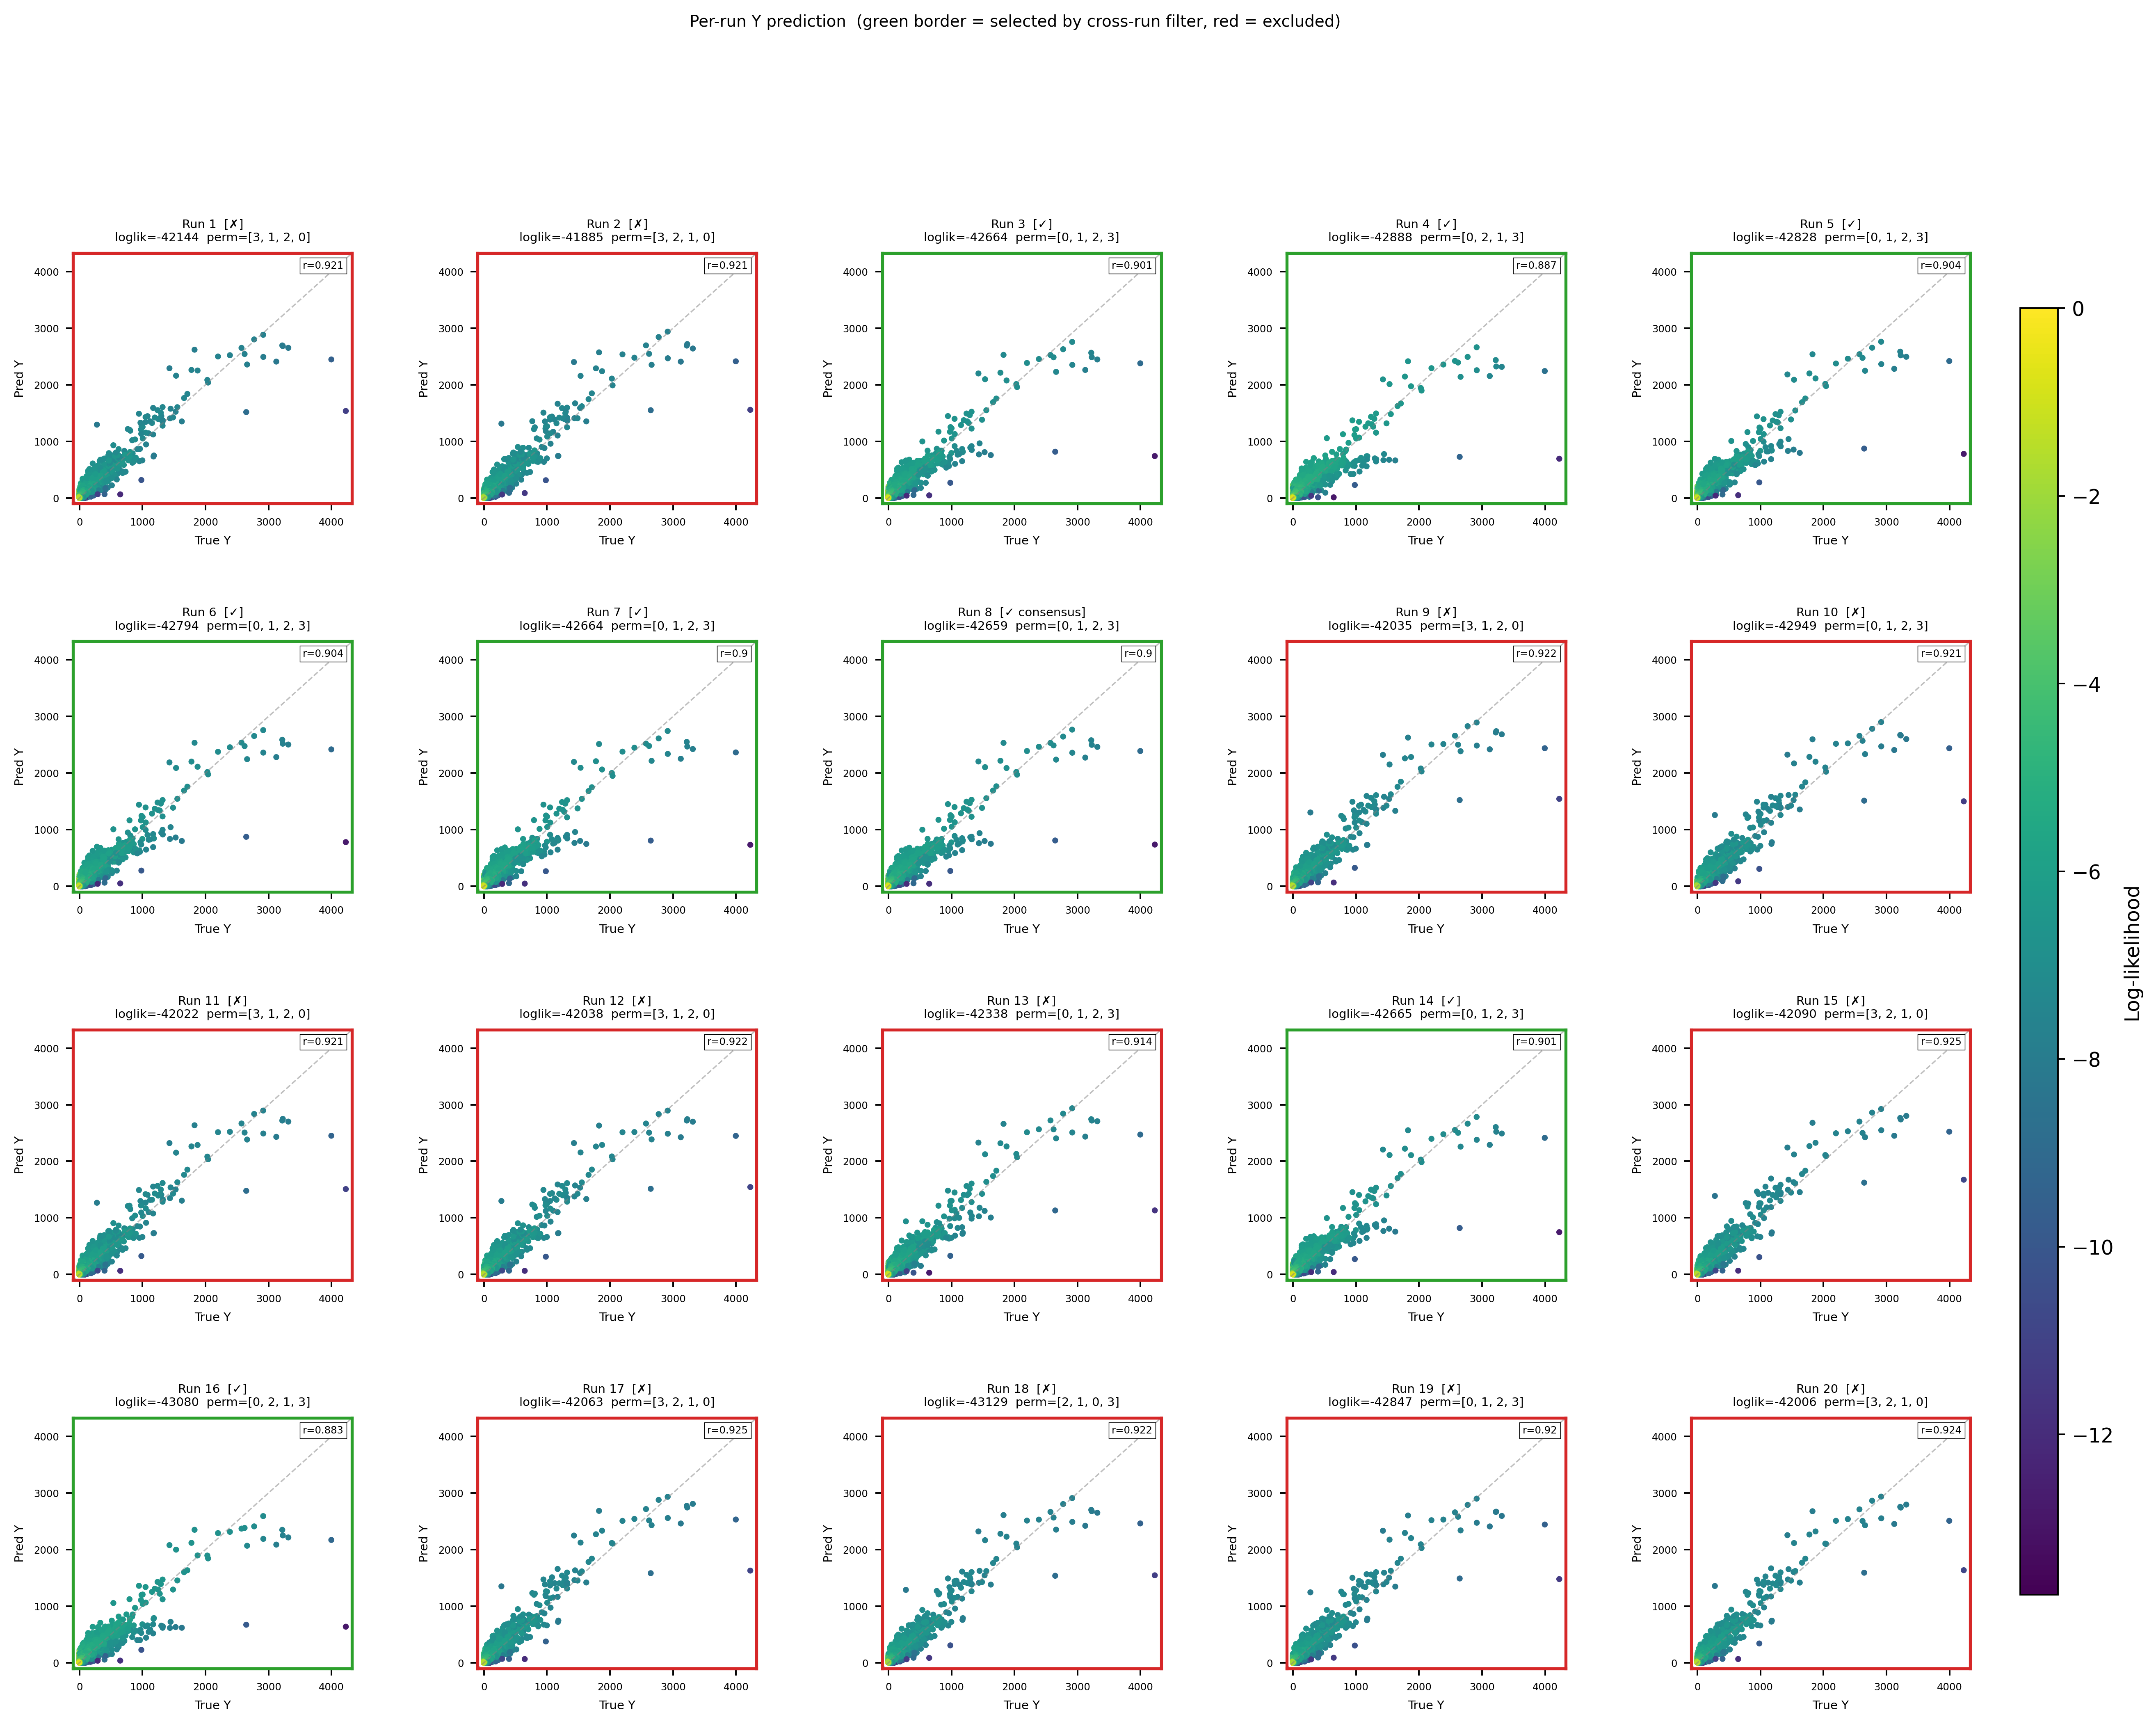
\includegraphics[width=\textwidth]{plots_paper/figure5_supp.png}
  \caption{%
    \textbf{Per-run predicted versus observed gene expression across all ten
    independent runs.}
    %
    \textit{Generation.}
    For each run, the within-run averaged $H$, $B$, and $n$ (cells per spot)
    were used to compute the predicted expression matrix
    $\hat{Y} = \mathrm{diag}(n) \cdot H \cdot B$, with per-section scaling
    applied to account for differing sequencing depths across the three
    tissue sections (P1.2, P2.4, P3.3).
    Each point in the scatter is one gene--spot observation; colour encodes
    the per-observation negative-binomial log-likelihood.
    The Pearson $r$ between $Y_{\mathrm{true}}$ and $\hat{Y}$ is annotated
    in each panel.
    Panels with a green border were selected by the consensus cross-run
    filter (runs~3--8); those with a red border were excluded (runs~1, 2,
    9, 10).
    Run~8 is additionally labelled as the consensus reference.
    %
    \textit{Result.}
    All runs — selected and excluded — achieve $r \approx 0.88$--$0.93$,
    confirming that every run fits the observed expression data well
    regardless of clone-label orientation.
    The marginal differences in fit confirm that the exclusion of runs~1,
    2, 9, and~10 is driven by label switching rather than by inferior
    predictive accuracy.%
  }
  \label{fig:figure5_supp}
\end{figure}
